
\documentclass{article}


\usepackage[english]{babel} % babel specifies the language
\usepackage[utf8]{inputenc} % this one is...confusing
\usepackage{amsmath} % amsmath allows many useful math tools
\usepackage{graphicx} % graphicx handles graphics
\usepackage{amssymb,amsmath,amsthm,amsfonts}
\usepackage{multicol,multirow}
\usepackage{calc}
\usepackage{ifthen}
\usepackage{gensymb}
\usepackage{wasysym}
\usepackage{subfig}
\usepackage{tcolorbox}
% The following is an optional package but I think it makes
% things look better.  "1in" is margin.  Delete this line to see
% the default LaTeX margins.
\usepackage[margin=1in]{geometry}
\newcommand{\ts}{\textsuperscript}

% The next three commands take arguments which get printed by
% the \maketitle command.  They should be self-explanitory.
\title{Operational Level Celestial Sight Planning \\
\large A Resource for Senior Deck Cruise}
\author{Joey Simone}
\date{\today} % \today will print the compile date


\begin{document}


\maketitle

% The \section command tells the compiler that you want to start
% a new section and the argument tells it the title of that
% section.  If you don't want a section to have a number then
% use \section* instead of \section.
\section*{Introduction}

% To make a paragraph in LaTeX just start typing on a new line.
% Make sure, however, that there is a blank line before and after
% the paragraph.  Try removing the line after "...useful skill."
% and see what happens to the output.
A common stumbling block for cadets doing their Celestial Project on cruise is planning their required star fixes and sun fixes. This document is made from my personal experiences making over a hundred sight plans on my own senior cruise. This Document provides the format, steps, and examples required for producing sight plans quickly and accurately in a way yielding to high quality fixes and communicating the planning information to fellow cadets. It is only necessary for one person to create a sight plan if it is posted in the Nav Lab, and so other people can set their alarms based on that plan.

For Star Fixes, both Morning and Evening, steps will be laid out for establishing the most correct twilight time for observations of stars and planets, the DR position at the recommended fix time, the selection of appropriate stars, the altitude and relative position of the moon and navigational planets, and creating a table and visual diagram for showing the others.

For the Sun Run Sun fix, this paper shows an effective way to determine estimated Local Time of LAN and the most satisfactory times to shoot the morning sun line and afternoon sun line.

% This section has a label on it.  Any use of \ref{sec:examples}
% will then print out the number of this section.
\section{The Math}\label{sec:examples}

% Subsections work similarly.  There is also a \subsubsection
% and more.
\subsection{The Sailings}

For the purpose of accuracy and rapid calculation, I like to use the sailings, and for this application I exclusively use the Mid Lat sailing. The additional accuracy rendered from the Mercator sailing is negligible on the short run of finding the morning position of the ship from the evening position. The "best" solution is to use the actual navigational chart, but you shouldn't do that if you're not on watch yourself, and the Nav Watch people will be doing this anyway. Universal Plotting Sheets are acceptable but they are the worst for this application. The margin of error in measurements of longitude is significant, it's not good to waste them on just making the sight plan, and you can do the sailings anywhere you can have your calculator and notebook. The mid lat sailing is accurate enough for the job, fast, and doesn't require tables or charts or plotting gear. With your TI-30xa and the most recent position slip (0800, NOON, or 2000), you can determine star time and vessel position. Here are the formulas you will use.

\begin{align*}
    D&=S\cdot T   &   L_2&=L_1+\ell   &   \lambda_2&=\lambda_1+DLo\\
    L_m&=\frac{L_1+L_2}{2}  &   \ell&=D\cos{C}  &   p&=D\sin{C}\\
    DLo&=\frac{p}{\cos{L_m}}    &\Longleftrightarrow     DLo&=\frac{D\sin{C}}{\cos{L_m}}\\
\end{align*}
Remembering that $C$ is Course Angle, the angle inside the triangle, not the angle clockwise from True North ($Cn$). To Convert from Cn to C, use the rules:

\begin{align*}
    &0<Cn<90 \to &C=Cn\\ &90<Cn<180 \to &C=180-Cn\\ &180<Cn<270 \to &C=Cn-180\\ &270<Cn<360 \to &C=360-Cn 
\end{align*}


\subsection{Phenomena}
For the Star Sights, you have to interpolate the twilight tables for your latitude to find the star time at the standard meridian, which then have to be adjusted for Longitude. The Meridian Passage is not sensitive to Latitude or Declination, and happens at the same time for the entire line of longitude, so the given times in the book must be adjusted for Longitude in the same way. There are two methods which are algebraically equivalent. Sam Pearson teaches the American method in class, I prefer the British method because it renders both the UT and the LT of the event, which you would need anyway.

\[\text{Almanac Time}+^{+W}_{-E}\frac{\lambda}{{15}\degree/\text{hr}}-\text{ZD}=\text{Local Time}\] 
The British Method gives the Universal Time of the event first, then you get Local Time by applying minus Zone Description.

\[\text{Almanac Time}+^{+W}_{-E}\left(\lambda-\frac{\text{ZD}\times15\degree}{1 \text{hr}}\right)=\text{Local Time}\] 
The American Method prioritizes finding the Local Time, then apply the zone description to get Universal Time.
The last of the mathematics is to find the LHA of Aries, here LHA\aries. The Almanac itself has instructions in the "Explanation" chapter.

\section{Star Sight Planning}
\subsection{Establishing Time and Position}
I have found that the most consistent way to organize the DR Positions in the AM and PM sight plan is with a table. Take the first line information from the position slip, for instance, when making the PM sight plan, use the Noon slip to get CSE, SPD, $L_1$, $\lambda_1$, ZD, and let $T_1$ be 1200hrs and $D_1$ be 0nm. 

% The table environment is very similar to the figure environment,
% as you can see.  The biggest difference between this and the
% figure is that the \includegraphics command has been replaced
% with the tabular environment.
\begin{table}[ht]
\centering
% Tabular is more complicated than \includegraphics.  The argument
% that is shown here as {l|r} controls a lot of things.  The letters
% control the spacing; try changing it to {l|c} or {l|l}.  The bar
% tells LaTeX to put a bar between columns.  Try {lc} or {|l|c|}.
% To add another column, simply add another letter like {l|r|r}.
\begin{tabular}{|l|l|l|l|}
% Within the tabular environment, column entries are separated by
% the & character and \\ represents the end of a row.  Use \hline
% between rows to print a line between them in the output.
\hline
Time (hhmm) & Latitude & Longitude & Distance (nm)\\ %<-- an entire row
\hline %<-- the horizontal line
$T_1$ & $L_1$ & $\lambda_1$ & 0 \\ % noon slip
\hline
$T_2$ & $L_2$ & -- & $D_2$ \\ % DR to soonest
\hline
$T_3$ & -- & $\lambda_3$ & $D_3$ \\ % Use interpolated T3
\hline
$T_4$ & $L_4$ & $\lambda_4$ & $D_4$ \\ % t4 from Arc to Time
\hline
% Note that the LAST row does not need a \\ after it.
\end{tabular}
\caption{Required Times, Positions, and Distances}
\label{tab:twilight positions}
\end{table}
All shots happen during Nautical Twilight, but some people are confused by the column to use. In the \emph{morning}, Shooting Time begins at Nautical Twilight, as per the Nautical Almanac, this time is BMNT for "Begin Morning Nautical Almanac". Shooting Time ends at the interpolated and corrected time of Civil Twilight, or BMCT. In the \emph{evening}, Shooting Time begins at the interpolated and corrected time in the Civil Twilight column, this time is End Evening Civil Twilight, EECT. Shooting time normally ends by End Evening Nautical Twilight

When selecting a time from the twilight column to be T2 for your table, select the earliest time in your pair of latitudes, so as to not overshoot. For instance, the date is Feb 07\ts{th} 2024, the DR Latitude is 38N.
\begin{center}
    \begin{tabular}{|l|cc|}
\hline
Lat&Naut&Civil\\
\hline
N40$\degree$&0603&0635\\
35$\degree$&0558&0628\\
\hline
\end{tabular}
\quad
\begin{tabular}{|l|cc|}
\hline
Lat&Civil&Naut.\\
\hline
N40$\degree$&1754&1826\\
35$\degree$&1800&183\\
\hline
\end{tabular}
\end{center}
In the morning, the table on the left applies, and we choose the soonest time in the Nautical column that applies to the Latitudes we are between, in this case 0558. In the evening, the table on the right applies, and we choose the soonest time in the Civil column that applies to the Latitudes we are between, in this case 1754.
\begin{enumerate}
    \item Adopt this time as $T_2$, DR out, and record $L_2$. Longitude is not needed in this step.
    \item Use $L_2$ to interpolate the column and find a most accurate center meridian time of the phenomena. For Latitudes greater than 40 North or South, more accuracy may be had using the Table 1 in the back of the Almanac, near the Lunar Sight Correction tables, although it may be necessary to perform a double interpolation of that table. The interpolated time is $T_3$
    \item DR to $T_3$ and record Longitude $\lambda_3$.
    \item Use \(T_3+^{+W}_{-E}\frac{\lambda_3}{{15}\deg/\text{hr}}-\text{ZD}=T_4\) or 
    \item DR to $T_4$ and record $L_4$ and $\lambda_4$
\end{enumerate}
From here on, $T_4$ is the (ship) time at which you should plan to be out on the Nav Lab or Bridge Wing with your sextant, notebook and pen, accurate wristwatch, and your red colored flashlight. For Clarity, $UT_4$ is the Universal (GMT) Time that you use to enter the Nautical Almanac and Air Sight Reduction Table.
\subsection{Writing the Sight Plan}
The fastest and most accurate resource for sight planning is the \emph{Sight Reduction Tables for Air Navigation, Vol. I}, sometimes called the Air Almanac by mariners, even though another book has that name. It can list the Name, Altitude, and Azimuth of the 7 best stars for shooting, and recommends 3 of them for a very good fix. All it wants is your (AP) Latitude and the LHA\aries for the time and place you will shoot. The procedure for finding AP Lat is exactly the same as in Sight Reduction, simply round $L_4$ to the nearest whole number. Table 4 in the back of the book gives instructions and numbers for finding the GHA of Aries to the nearest minute of arc in a ten year period. The book labeled epoch 2025 is good for years 2021-2029. Use $UT_4$ to find GHA\aries and then use $\text{GHA}\aries^{+E}_{-W}\lambda_4=\text{LHA}\aries$ and round to the nearest whole number. Pages in the table are labeled by Latitude, and then find the row with the corresponding LHA\aries.
\begin{figure}[h]
    \centering
    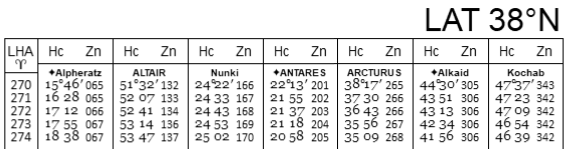
\includegraphics[width=0.5\linewidth]{249excerpt.png}
    \caption{Excerpt from Pub 249, Page for L38N}
\end{figure}\\
Stars listed in all upper case, such as SIRIUS, are among the twenty brightest stars, brighter than magnitude 1.5. On each line, three stars are marked with a diamond symbol $\blacklozenge$. These are best suited, among the seven available, for a fast three-star fix with wide crossing angles among the resulting lines of position. Shoot those first unless clouds or viewing angle limitations rule them out. 

If a two-star fix is preferred, ignore the diamonds, and choose the most convenient pair from the seven that are bright, easily-identified, and separated by at least 45\degree\ and not more than 135\degree\ in azimuth, preferably near 90\degree\ apart. For each star, the Main Table provides the un-refracted altitude above the true horizon, referred to in the intercept method as Hc, and also the true azimuth (non-magnetic compass direction) measured clockwise in degrees from true north, labeled Zn.
\subsection{Use of the RUDE Star Finder}
I find that my accuracy with the star finder is reduced for main stars like are covered in the Pub 249 table, but in situations where the Air Nav Table is not available, you can get much the same information, with less accuracy. The blue disks are reversible, with *5N on one side and *5S on the other. Each disk is good for 5 degrees on either side, so if your latitude is 38N, use the disk labeled 35N. Find the LHA\aries from the Nautical Almanac in the usual way, and put the blue disk on the white disk so that the arrow points to the right number for LHA on the bottom. Look at the stars about 45 degrees up the disk (middle altitude) and find stars which are well distributed in azimuth, 120 degrees between them is ideal. Stars with big circles are brighter, stars with tiny dots are dimmer, and the peg at the center of the disk is Polaris (in the Northern Hemisphere)

Where the Star Finder shines is the ability to display the Minor Stars, the Navigational Planets, and the Moon. Use the red disk, the Right Ascension of the body (\(\text{RA}=360\degree-\text{SHA}\)) and the Declination of the same body at $UT_4$. If you desire to use the moon, \(\text{RA\leftmoon}=360-\text{GHA\leftmoon}+\text{GHA\aries}\)

Play around with this. Once you have drawn all the planets and moon on your star finder, you can scroll the blue disk back and forth to find, for instance, the LHA Aries associated with moonrise and moonset, or the meridian passage of a planet, then you can work backwards with your $\lambda_4$ and your almanac to find what time in UT and LT that will happen. It's like having the world's cheapest planetarium. 
\subsection{Putting it all together}
Now that you know all of this stuff, the most helpful thing you can do is to distill it into a format that is understandable to your friends, and post it in the nav lab. If someone wants to know for what time they should set their alarm in the morning, the ship time and universal time of BMNT is posted on your sight plan. The ship's direction and speed from the position slip and the DR Lat and Long have to be on your plotting sheet anyway for your work to be counted, so include it on the sight plan. The most important thing is to include a brief table with the name, altitude and azimuth of each body.

\begin{table}[hb]
    \centering
 June 26 AM Sight Plan\\
    ZD=+9, CSE 042, SPD 15.2,
    Reckoned from 25 Jun 2023, 2000 POSN SLIP\\
    UT BMNT 1342, LT BMNT 0442, 0442 DR Posn: L$31\degree\ 26.4'\text{N}, \lambda146\degree\ 43'$W\\
    \begin{tabular}{|cl|cc|}
        \hline
        Symbol & Name & Hc & Zn \\
        \hline
        $\blacklozenge$  & Mirfak & $30\degree16'$ & 047\\
        $\blacklozenge$ & FOMALHAUT & $28\degree29'$ & 168 \\
        $\blacklozenge$  & VEGA & $46\degree01'$ & 295 \\
        $\star$ & Hamal & $37\degree31'$ & 083 \\
        $\star$ & Diphda & $28\degree54'$ & 138 \\
        $\star$ & ALTAIR & $50\degree41'$ & 243 \\
        $\star$  & Kochab & $24\degree25'$ & 344 \\
        \rightmoon & MOON & NOT & AVAILABLE \\ 
        \venus  & VENUS & NOT & AVAILABLE \\ 
        \mars  & MARS & NOT & AVAILABLE \\ 
        \jupiter  & JUPITER & $30\degree$ & 090 \\
        \saturn  & SATURN & $48\degree$ & 171 \\ \hline
    \end{tabular}
    \caption{Created from a real sight plan I made on the TSGB}
    \label{tab:digitzed example}
\end{table}
\pagebreak
\subsection{Example}
\begin{figure}[h]
    \centering
    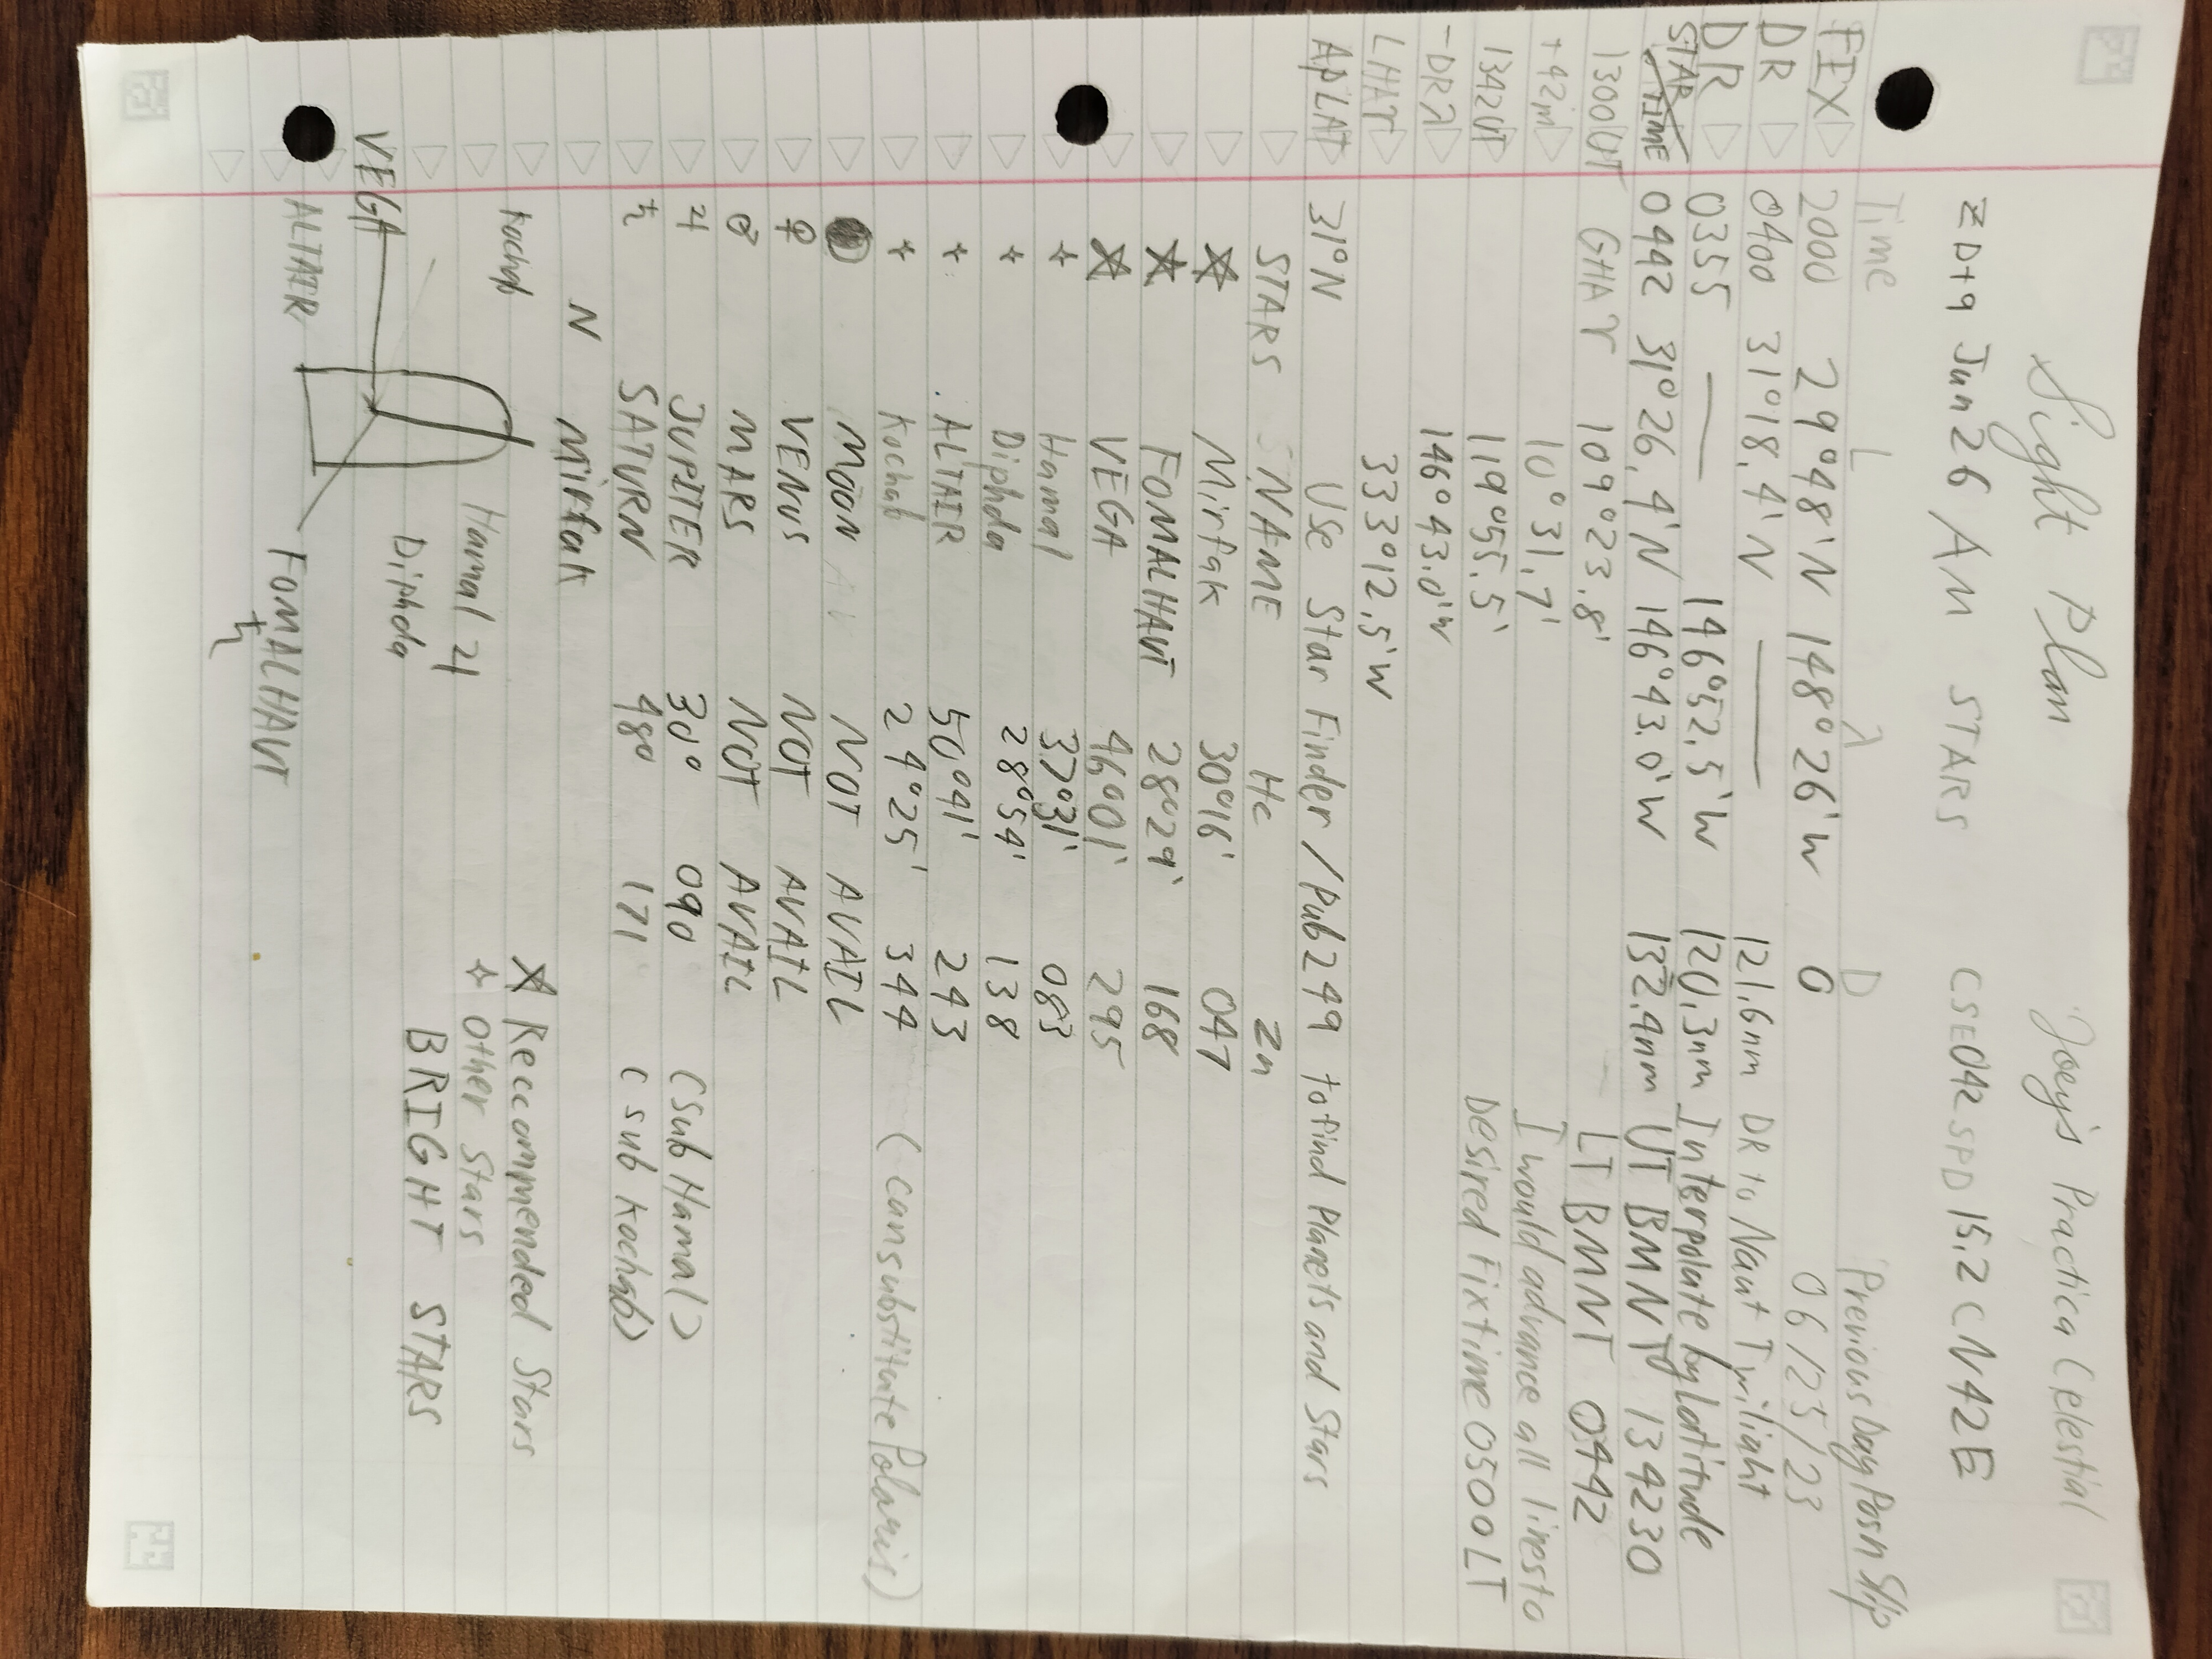
\includegraphics[width=1\linewidth,angle=90,origin=c]{IMG20240206151513.jpg}
    \caption{Handmade Sight Plan with all tables and drawings.}
    
    
\end{figure}
\pagebreak
\section{Daylight Fixes}
\subsection{Making the Plan}
The process for creating good sight geometry in your daylight running fixes is much more brief, and you are already a little acquainted with the process from the second unit of Pearson's class. As before, we want to find the UT and LT of LAN using "Mer. Pass." from the Almanac and use the 0800 POSN slip to establish CSE, SPD, ZD, $L_1$, $\lambda_1$, and let $T_1$ be 0800 and $D_1$ be 0nm.

Create the table.
\begin{table}[h]
\centering
\begin{tabular}{|l|l|l|l|}

\hline
Time (hhmm) & Latitude & Longitude & Distance (nm)\\
\hline
$T_1$ & $L_1$ & $\lambda_1$ & 0 \\ % 0800 slip
\hline
$T_2$ & --- & $\lambda_2$ & $D_2$ \\ % DR to soonest
\hline
$T_3$ & $L_3$ & --- & $D_3$ \\ % corrected T3
\hline
% Note that the LAST row does not need a \\ after it.
\end{tabular}
\caption{Required Times, Positions, and Distances}
\label{tab:sunlight positions}
\end{table}
\begin{enumerate}
    \item Set "Mer. Pass." from the correct day in the Almanac as $T_2$, DR to $T_2$ and record $\lambda_2$ only.
    \item \(T_2+^{+W}_{-E}\frac{\lambda_2}{{15}\degree/\text{hr}}-\text{ZD}=\text{LT LAN}\)
    \item Let LT LAN be $T_3$. DR to $T_3$ and record $L_3$. LT LAN + ZD = UT LAN ($UT_3$)
    \item Use $UT_3$ to find Dec \astrosun\ (Sun)
    \item Find the Absolute Difference of \((\text{Lat}\sim \text{Dec})\), which is to say $L-D$ if Latitude and Declination are same hemisphere and $L+D$ if contrary hemispheres.
    \item This is the same thing as your predicted co-alt\footnote{Pearson calls it Zenith Distance, but I don't like that because it also abbreviates to ZD, like zone description.}, or \(90-\text{Ho}\).
    \item Multiply your co-alt in degrees by \(\frac{4\text{min}}{1\degree}\) to get difference of time, which I'm calling \(\Delta T\)
    \item The best time to shoot your AM sun line is \(T_3-\Delta T\), and your PM sun line time is \(T_3+\Delta T\).
\end{enumerate}
Then, a much shorter Sight Plan can be created, posted, shared with friends, and hastily copied down into pocket notebooks in the chow line.
\begin{tcolorbox}
\begin{center}
    Sun Noon Sun Sight Plan
    
ZD$=+10$, CSE 237 SPD 10, Reckoned from 0500 Star Fix in POSN L$00\degree39.1'\text{N},\lambda148\degree49'$W
\begin{itemize}
    \item Shoot AM sun line at 1030
    \item LAN occurs at 1156
    \item Shoot PM sun line at 1322
\end{itemize}
Recommend Advance/Retard all lines to 1200.
\end{center}
\end{tcolorbox}
\pagebreak
\subsection{Example}
\begin{figure}[h]
    \centering
    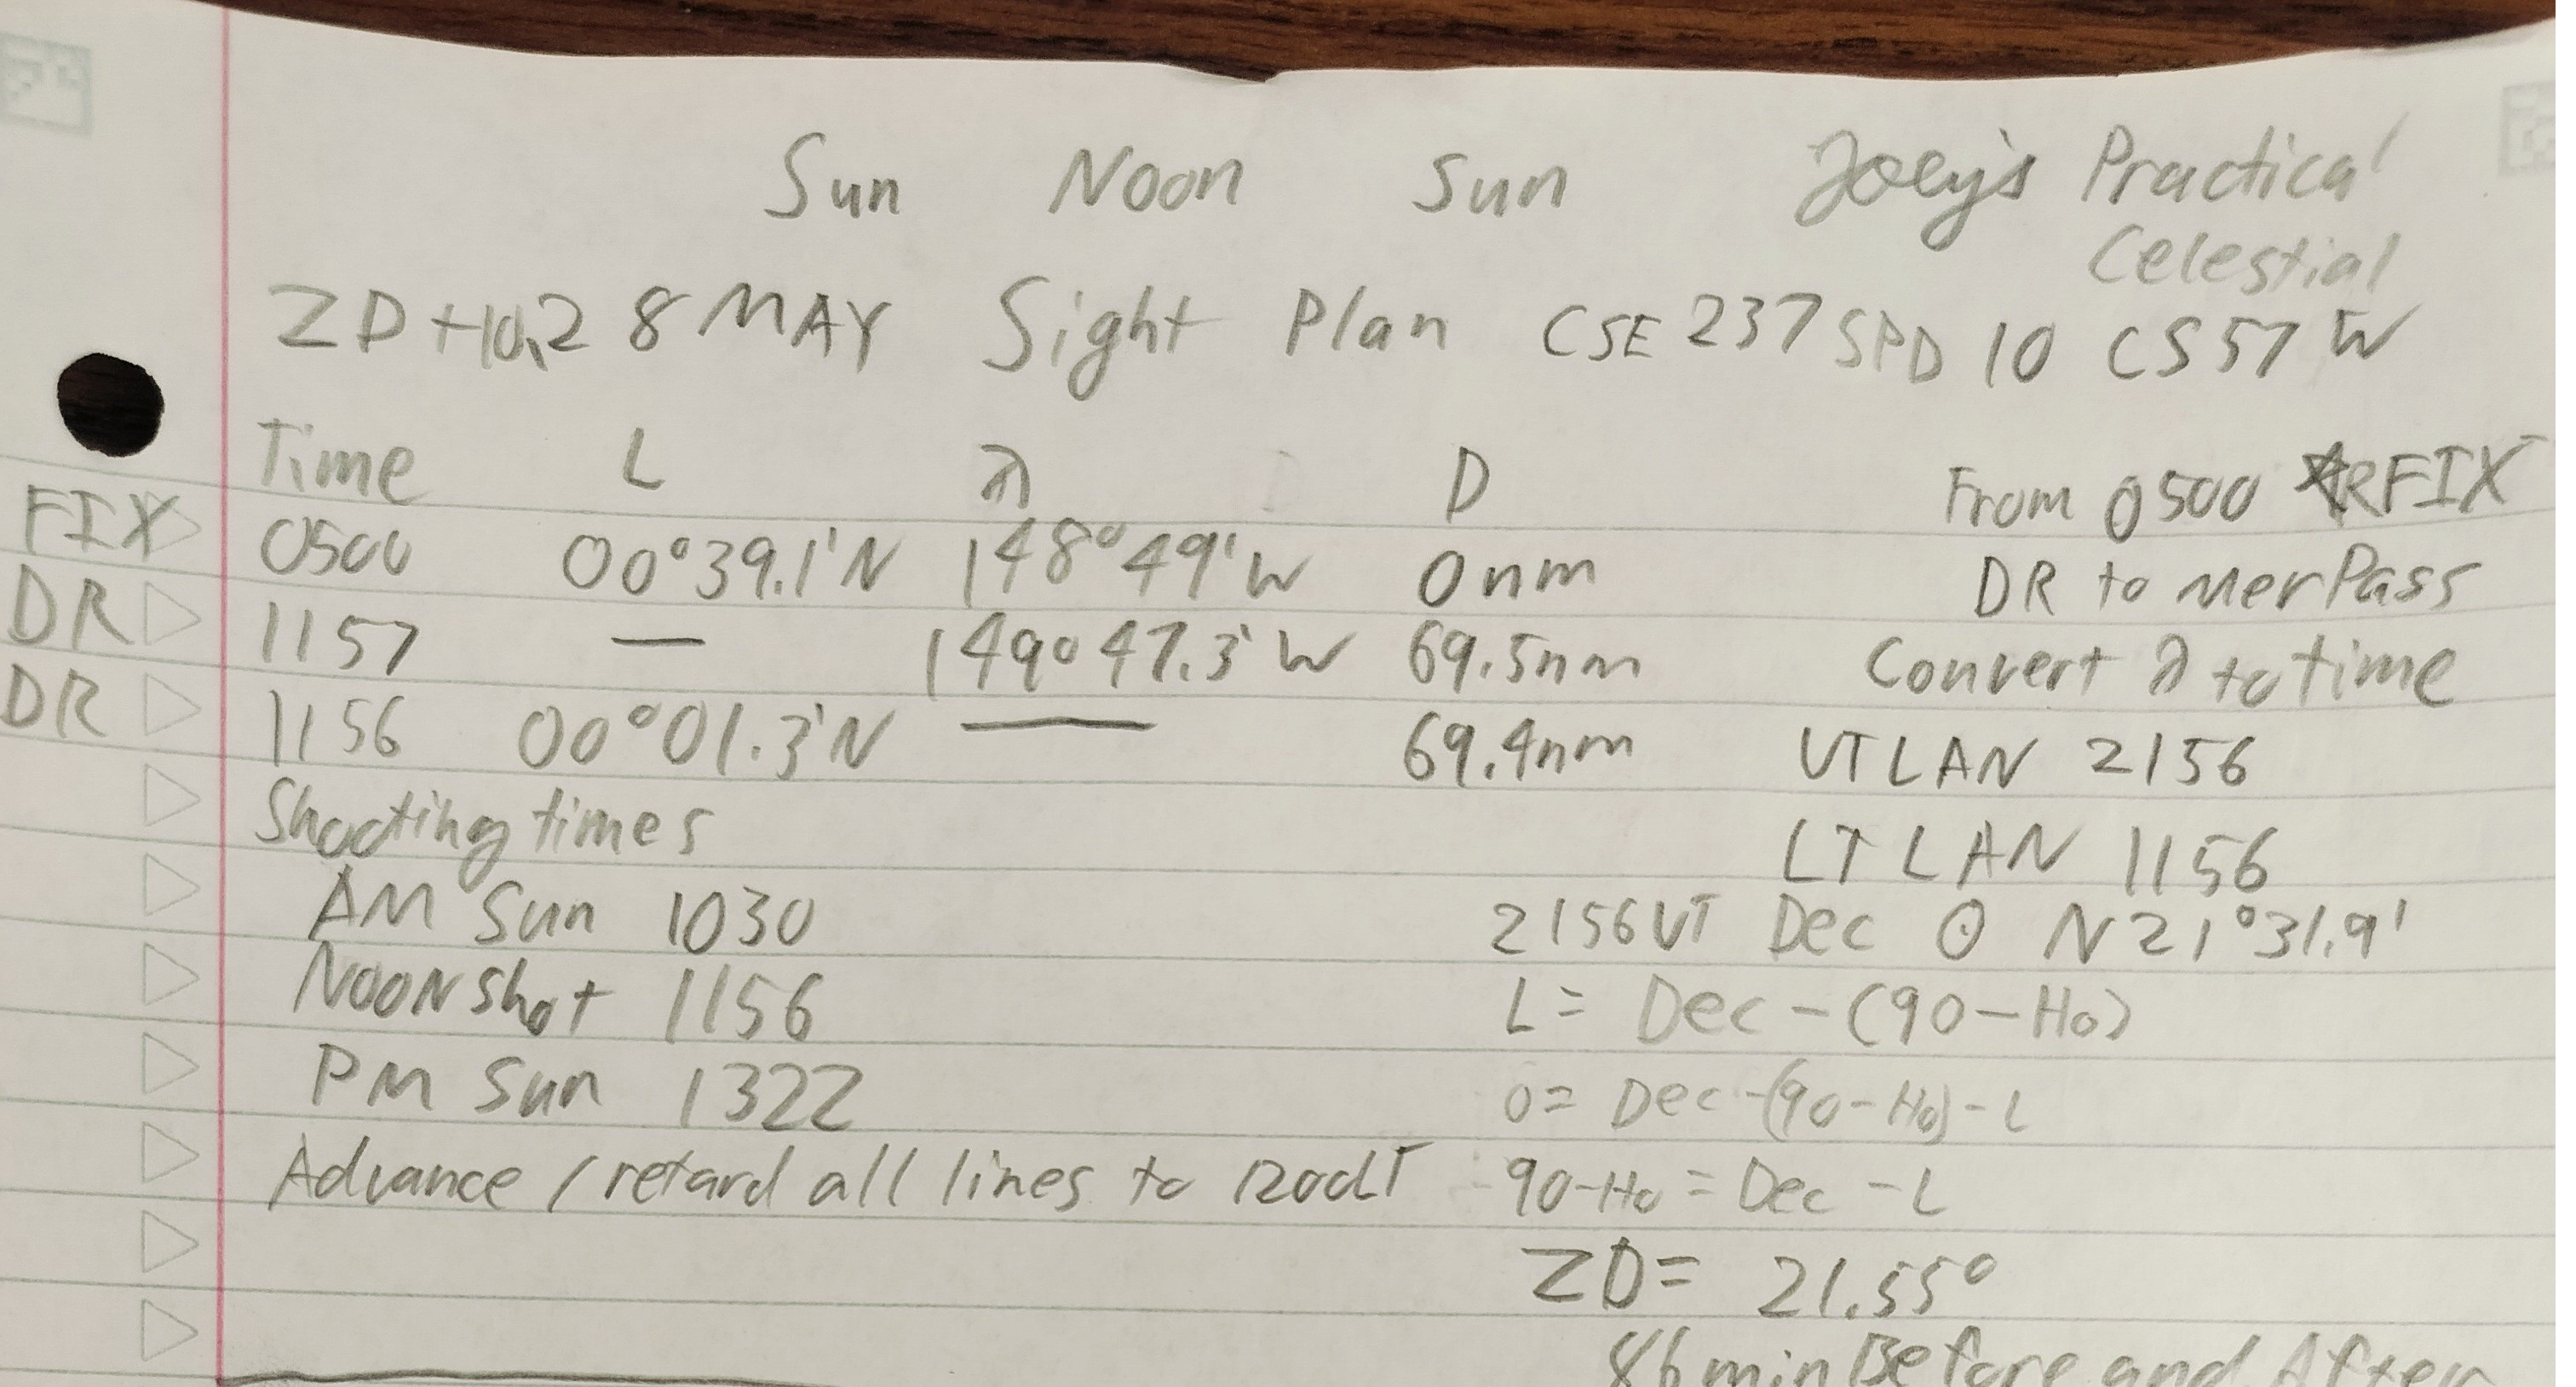
\includegraphics[width=1\linewidth]{IMG20240206151605~3.jpg}
    \caption{A recreated sight plan from when we crossed the equator going southwest at noon.}
\end{figure}
\section*{Conclusion}
There is always more to be learned in the art of celestial navigation. Omitted from this handout are the instructions for the use of Tables 1 and 2 in the back of the almanac, instructions for calculation of Moonrise and Moonset, instructions on planning daylight three body fixes with the Moon, The Sun, and Venus all at once, the use of the Star Finder to precalculate Sun Azimuth for perfect 60-60-60 triangles, and the calculations in pub 249 that allow the navigator to advance and retard star LOPs non graphically. This paper is just for helping you get the Sun and Star fixes that the instructors want you to get, and for helping you formulate and communicate sight plans to your fellows in a productive and consistent way. Besides, if you're interested in the other stuff, trying to figure it out on your own is one of the most rewarding and exciting parts of this ancient discipline. Don't let me have all the fun.

\begin{center}
    Good Luck, happy shooting, don't get arrested in port.
\end{center}
\end{document}
